\documentclass[12pt]{article}

\usepackage{float}
\usepackage[pdftex]{graphicx} 
\graphicspath{{../img/}}
\DeclareGraphicsExtensions{.pdf,.jpeg,.png,.jpg} 

\usepackage{listings}
\lstset{language=Python, keywordstyle=\color{blue}, stringstyle=\color{olive}, breaklines=true, showstringspaces=false, float, tabsize=2}
\usepackage{xcolor}
\usepackage{textcomp}
\usepackage{subcaption}

%opening
\title{Laboratory exercise no. 2: Heat transfer simulation}
\author{Piotr Gawry\'s $<pgawrys2@gmail.com>$}

\begin{document}

\maketitle

\section{Introduction}

The goal of this laboratory is to implement simulation of heat transfer for three plates each made of different metal:
\begin{enumerate}
	\item Alumina.
	\item Cooper.
	\item Stainless Steel.
\end{enumerate}

During the course of the laboratory we will also implement initial and boundary conditions, test numerical stability and calculate spacial and temporal temperature distribution in the plate for boundary conditions of type 1 and 2.

\section{Implementation}

First, we will write function containing relevant physical parameters of each metal:

\lstinputlisting[language=Matlab, caption = {Choosing material}, frame=single]{../source_code/choose_material.m}

This will allow us to reuse it instead of repeating it every time. \\

The metal plate has heater attached in the middle. We assume that both heater and the plate have square shape. The side of the heater is assumed to be \textit{0.05 m} and the side of the plate is \textit{0.2 m}.

\subsection{Equation}

We will need to use equation describing our mathematical model:

\lstinputlisting[language=Matlab, caption = {Equation describing mathematical model}, frame=single]{../source_code/equation.m}

The reason for using \textit{0.075} in the equation is that it is distance between the side of the plate and the heater in the straight line and before applying the equation we need to verify our current coordinates.

This function will also continuously plot simulation.

\subsection{Boundary condition type 1}

We consider two different boundary conditions (\textbf{type 1} and \textbf{type 2}) which also can be described with appropriate functions.

Regarding type 1 -- area having contact with the heater has a constant temperature of 80\textdegree{C} while the edge of plate has constant temperature of 10\textdegree{C}. The rest is calculated using equation implemented in the previous subsection.

\lstinputlisting[language=Matlab, caption = {Boundary condition of type 1}, frame=single]{../source_code/bc_type1.m}

We can pull everything together and add initial parameters to run this simulation:

\lstinputlisting[language=Matlab, caption = {Heat transfer for boundary condition of type 1 for Alumina}, frame=single]{../source_code/heat_transfer.m}

\begin{figure}[H]
	\centering
	\begin{subfigure}[b]{0.475\textwidth}
		\centering
		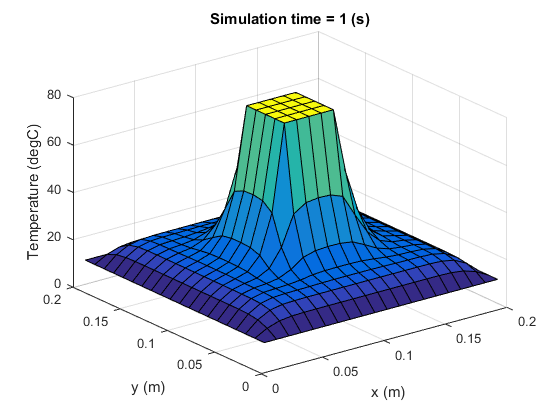
\includegraphics[width=\textwidth]{b_1}
		{{\small Simulation time: 1 (s)}}    
	\end{subfigure}
	\hfill
	\begin{subfigure}[b]{0.475\textwidth}  
		\centering 
		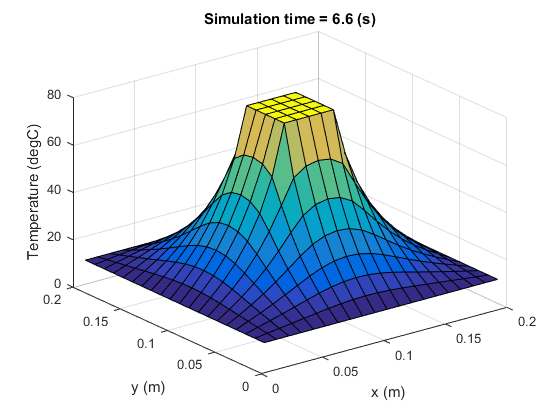
\includegraphics[width=\textwidth]{b_1a}
		{{\small Simulation time: 6.6 (s)}}    
	\end{subfigure}
	\vskip\baselineskip
	\begin{subfigure}[b]{0.475\textwidth}   
		\centering 
		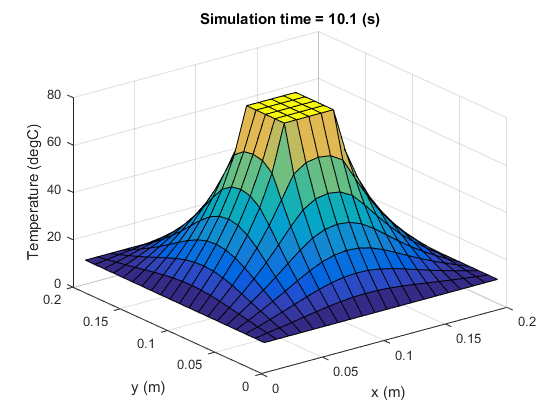
\includegraphics[width=\textwidth]{b_1b}
		{{\small Simulation time: 10.1 (s)}}    
	\end{subfigure}
	\quad
	\begin{subfigure}[b]{0.475\textwidth}   
		\centering 
		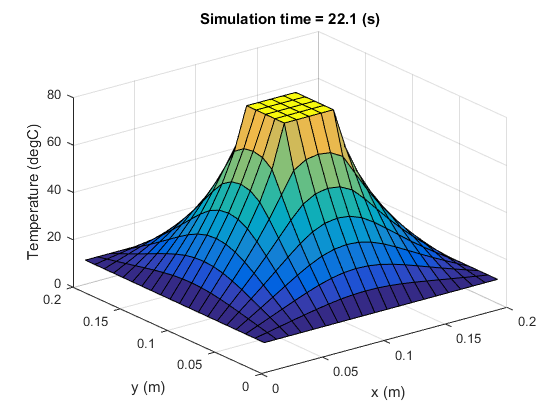
\includegraphics[width=\textwidth]{b_1c}
		{{\small Simulation time: 22.1 (s)}}    
	\end{subfigure}
	{\small Temperature distribution in heat transfer simulation with boundary of type 1 for Alumina} 
\end{figure}

The resulting plot shows that it starts with heat only around the heater but in just few seconds the area around it becomes warmer up to specific point after it remains stable regardless of time.

\subsection{Numerical stability}
Numerical stability usually means that for small disruptions in data the results will also notice small disruptions which is generally desired property as opposed to big changes.

We can find out when our model becomes unstable for Alumina using different values of time steps and spatial resolutions which means changing dt, dx and dy values.

\begin{figure}[H]
	\centering
	\begin{subfigure}[b]{0.475\textwidth}
		\centering
		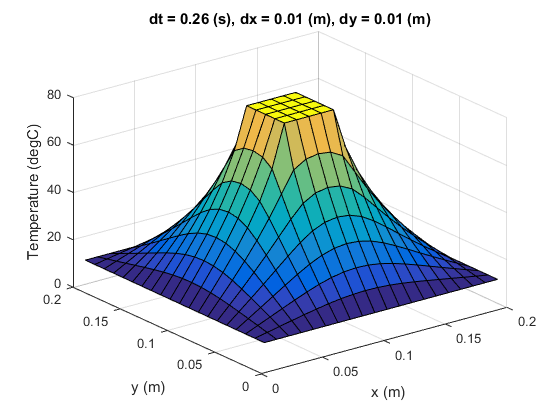
\includegraphics[width=\textwidth]{s_026}
		{{\small Time step: 0.26 (s)}}    
	\end{subfigure}
	\hfill
	\begin{subfigure}[b]{0.475\textwidth}  
		\centering 
		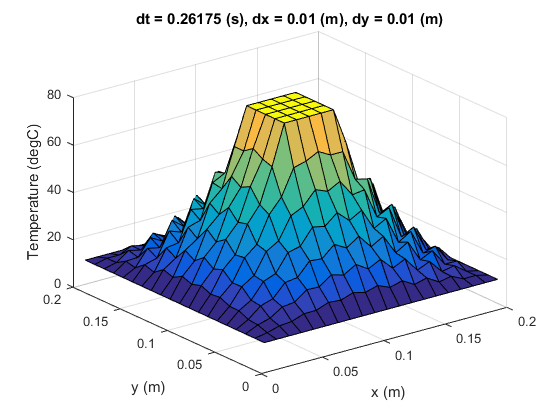
\includegraphics[width=\textwidth]{s_026175}
		{{\small Time step: 0.26175 (s)}}    
	\end{subfigure}
	\vskip\baselineskip
	\begin{subfigure}[b]{0.475\textwidth}   
		\centering 
		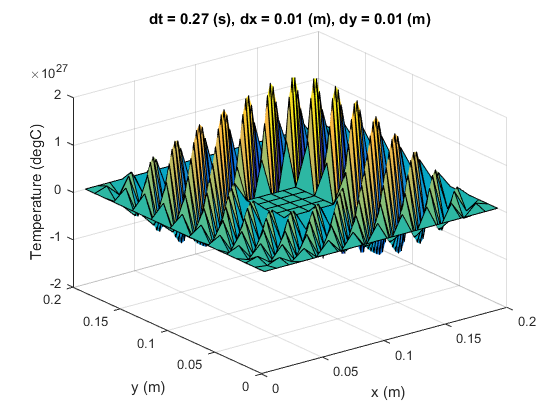
\includegraphics[width=\textwidth]{s_027}
		{{\small Time step: 0.27 (s)}}    
	\end{subfigure}
	\quad
	\begin{subfigure}[b]{0.475\textwidth}   
		\centering 
		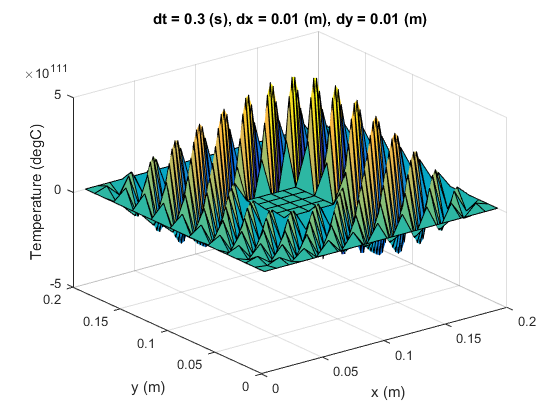
\includegraphics[width=\textwidth]{s_03}
		{{\small Time step: 0.3 (s)}}    
	\end{subfigure}
	{\small Stability tests for different time steps. We can observe that model is starting to lose stability for time steps higher than 0.26 s.} 
\end{figure}

\begin{figure}[H]
	\centering
	\begin{subfigure}[b]{0.475\textwidth}
		\centering
		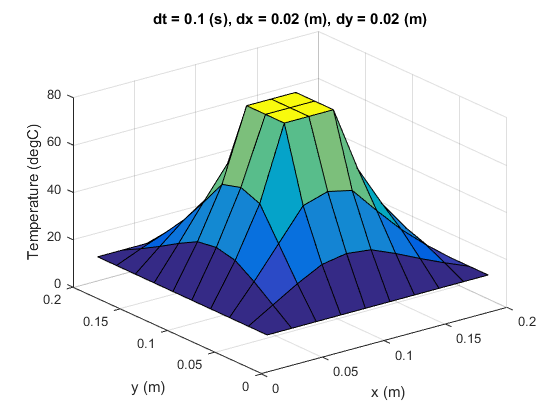
\includegraphics[width=\textwidth]{s0202}
		{{\small Spatial steps: 0.02 (m)}}    
	\end{subfigure}
	\hfill
	\begin{subfigure}[b]{0.475\textwidth}  
		\centering 
		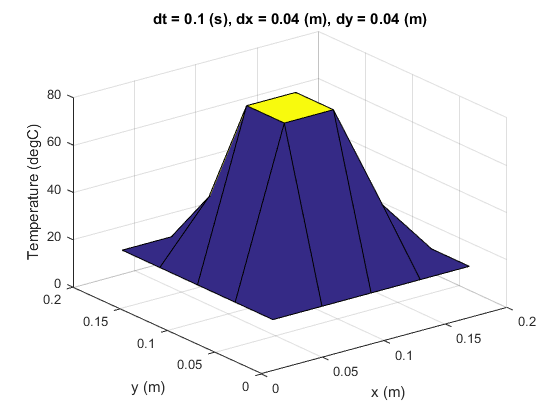
\includegraphics[width=\textwidth]{s0404}
		{{\small Spatial steps: 0.04 (m))}}    
	\end{subfigure}
	\vskip\baselineskip
	\begin{subfigure}[b]{0.475\textwidth}   
		\centering 
		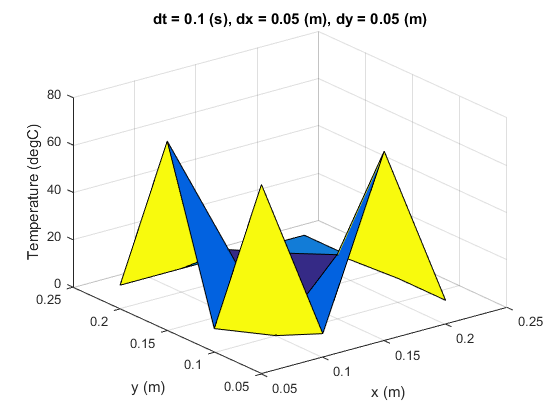
\includegraphics[width=\textwidth]{s0505}
		{{\small Spatial steps: 0.05 (m)}}    
	\end{subfigure}
	\quad
	\begin{subfigure}[b]{0.475\textwidth}    
	\end{subfigure}
	{\small \\ Stability tests for different spatial resolutions. The model is very quickly losing details but it is to be expected and for dx and dy = 0.04 (m) shape stays about the same. Stability loss occurs somewhere between 0.04 (m) and 0.05 (m).} 
\end{figure}

\subsection{Boundary condition type 2}
In this case we assume a constant power of the heater equal to 100W during the first 10s of the simulation. It is switched off later.

Implementation is very similar to previous boundary but we add part responsible for turning heater off.

\lstinputlisting[language=Matlab, caption = {Heat transfer for boundary condition of type 2}, frame=single]{../source_code/bc_type2.m}

We can run it the same way we did last time but we need two additional parameters:

\begin{lstlisting}[language=Matlab, caption = {Additional parameters for boundary condition of type 2}, frame=single]
% plate thickness
h = 0.002;
% heater power 
P = 100;
\end{lstlisting}

We will compare results for Alumina and Cooper.
\begin{figure}[H]
	\centering
	\begin{subfigure}[b]{0.475\textwidth}
		\centering
		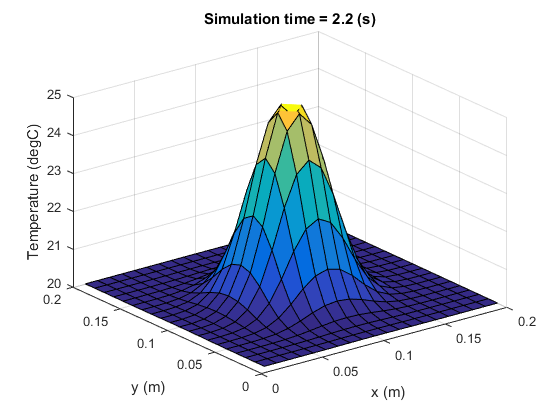
\includegraphics[width=\textwidth]{b2aA}
		{{\small Simulation time: 2.2 (s)}}    
	\end{subfigure}
	\hfill
	\begin{subfigure}[b]{0.475\textwidth}  
		\centering 
		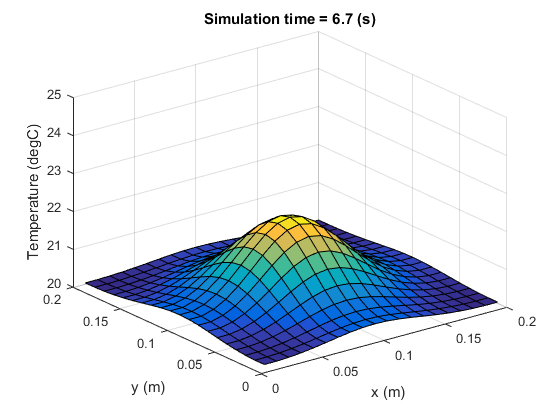
\includegraphics[width=\textwidth]{b2bA}
		{{\small Simulation time: 6.7 (s)}}    
	\end{subfigure}
	\vskip\baselineskip
	\begin{subfigure}[b]{0.475\textwidth}   
		\centering 
		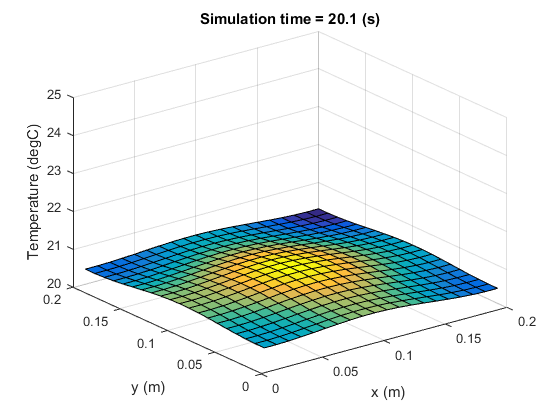
\includegraphics[width=\textwidth]{b2cA}
		{{\small Simulation time: 20.1 (s)}}    
	\end{subfigure}
	\quad
	\begin{subfigure}[b]{0.475\textwidth}   
		\centering 
		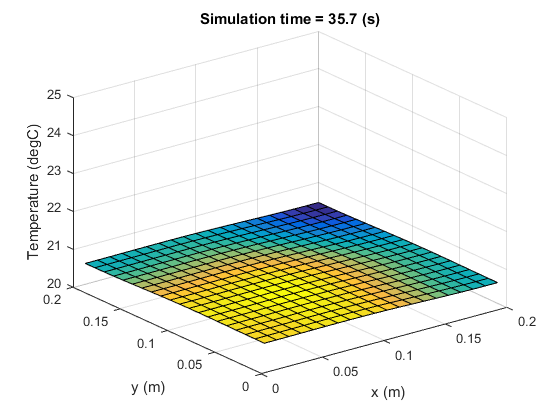
\includegraphics[width=\textwidth]{b2dA}
		{{\small Simulation time: 35.7 (s)}}    
	\end{subfigure}
	{\small Heat transfer for boundary condition of type 2 using Alumina plate} 
\end{figure}

\begin{figure}[H]
	\centering
	\begin{subfigure}[b]{0.475\textwidth}
		\centering
		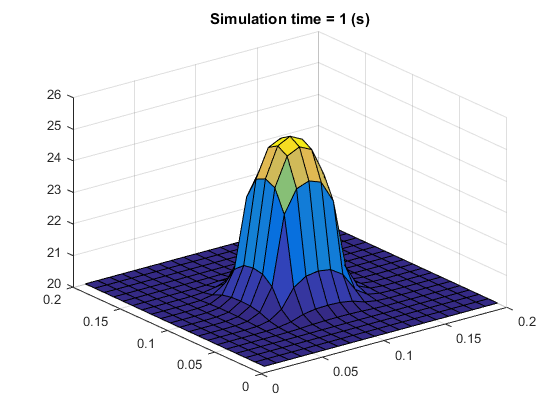
\includegraphics[width=\textwidth]{b2aC}
		{{\small Simulation time: 1 (s)}}    
	\end{subfigure}
	\hfill
	\begin{subfigure}[b]{0.475\textwidth}  
		\centering 
		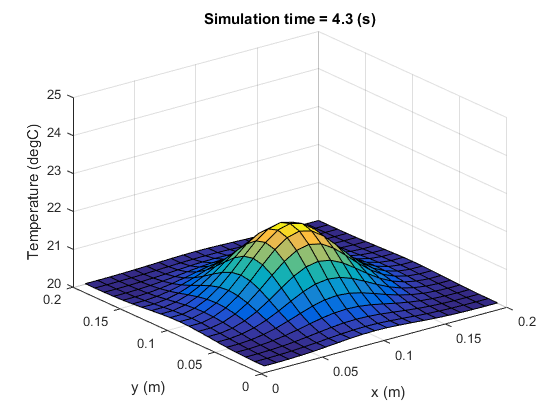
\includegraphics[width=\textwidth]{b2bC}
		{{\small Simulation time: 4.3 (s)}}    
	\end{subfigure}
	\vskip\baselineskip
	\begin{subfigure}[b]{0.475\textwidth}   
		\centering 
		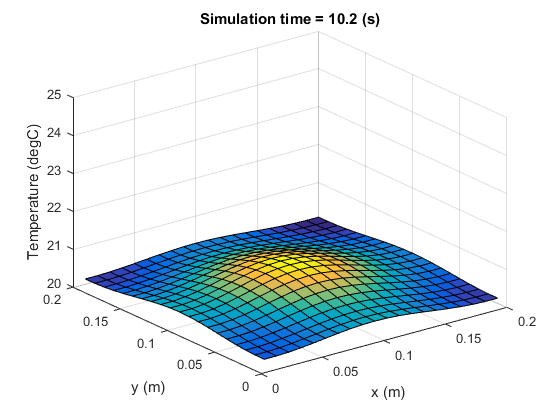
\includegraphics[width=\textwidth]{b2cC}
		{{\small Simulation time: 10.2 (s)}}    
	\end{subfigure}
	\quad
	\begin{subfigure}[b]{0.475\textwidth}   
		\centering 
		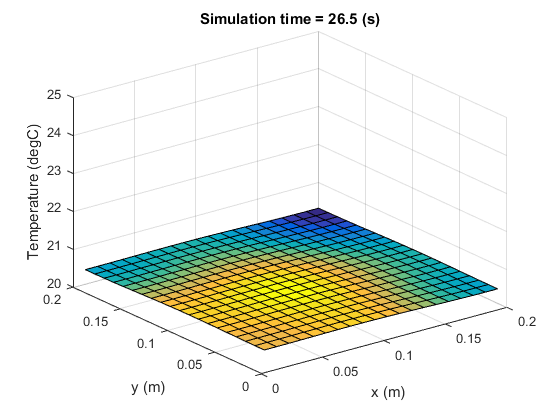
\includegraphics[width=\textwidth]{b2dD}
		{{\small Simulation time: 26.5 (s)}}    
	\end{subfigure}
	{\small Heat transfer for boundary condition of type 2 using Cooper plate} 
\end{figure}

In both cases it starts with rapid increase in temperature around heater area and then it dissipates (more about it in the later subsection) but the process is significantly faster for Cooper. The plate reaches similar steady state after around 26.5 seconds in comparison to 35.7 seconds in case of Alumina. This makes sense because Cooper's thermal conductivity is much bigger than Alumina's.

\subsection{The comparison of final temperature increment for 2-nd type of boundary condition with theoretical heat balance calculation.}

We can compare \textit{steady state} which can be observed at the last sub figures in the previous subsection to theoretical heat balance. To calculate steady state we can either check heat changes between time steps or do it empirically. Either way it occurs after about 35.7 seconds for Alumina.

If we saved our current state, we can simply calculate the value:

\begin{lstlisting}[language=Matlab, caption = {Heat balance for simulation}, frame=single]
% we take maximum from T and subtract starting temperature
max(max(T(:, :, t))) - 20
\end{lstlisting}
In our case it results in around 0.59\textdegree{C}.

Theoretical heat balance can be calculated from the equation:
\begin{equation}
\Delta T = \frac{P \cdot t}{c_w \cdot A^2 \cdot h \cdot \rho}
\end{equation}

Which is around 0.514\textdegree{K} for Alumina with A = 0.2 and h = 0.002.

Results are not quite the same but pretty similar.

\subsection{Heat dissipation}
It occurs when an object that is hotter than other objects is placed in an environment where the heat is transferred to colder objects and the environment itself. To put it simply -- it refers to heat loss from a hotter body to colder one. Implementation can be found below:

\lstinputlisting[language=Matlab, caption = {Heat dissipation for Alumina}, frame=single]{../source_code/heat_diss.m}

\begin{figure}[H]
	\centering
	\begin{subfigure}[b]{0.475\textwidth}
		\centering
		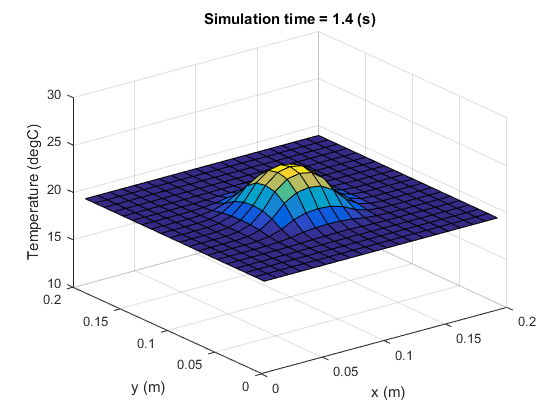
\includegraphics[width=\textwidth]{heat_diss}
		{{\small Simulation time: 1.4 (s)}}    
	\end{subfigure}
	\hfill
	\begin{subfigure}[b]{0.475\textwidth}  
		\centering 
		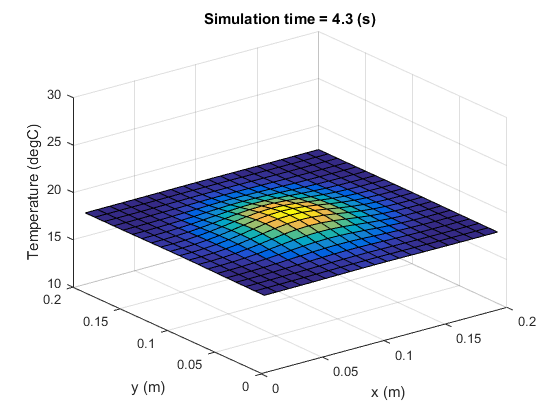
\includegraphics[width=\textwidth]{heat_dissB}
		{{\small Simulation time: 4.3 (s)}}    
	\end{subfigure}
	\vskip\baselineskip
	\begin{subfigure}[b]{0.475\textwidth}   
		\centering 
		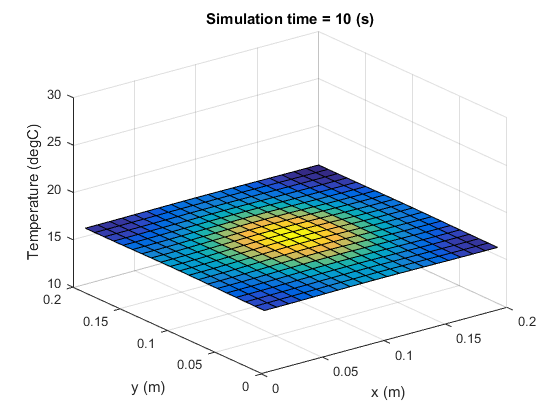
\includegraphics[width=\textwidth]{heat_dissC}
		{{\small Simulation time: 10 (s)}}    
	\end{subfigure}
	\quad
	\begin{subfigure}[b]{0.475\textwidth}   
		\centering 
		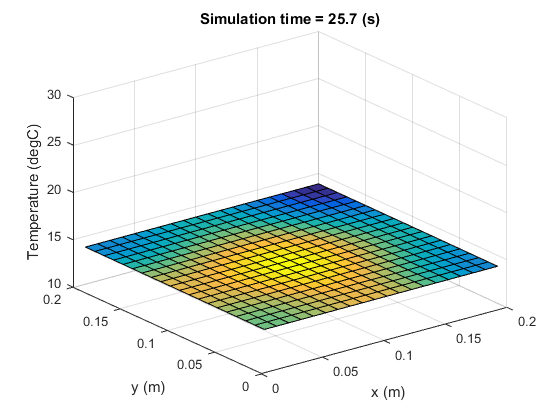
\includegraphics[width=\textwidth]{heat_dissD}
		{{\small Simulation time: 25.7 (s)}}    
	\end{subfigure}
	{\small Heat dissipation for Alumina} 
\end{figure}

The heater starts surrounded by cold objects transferring its heat with time. We can see that overall level of heat in the environment (including heater) is decreasing which complies to the second law of thermodynamics. 

\section{Conclusion}

During this laboratory we have successfully implemented simulation of heat transfer for several metals using two different boundary conditions. 

We have visualized temporal evolution of spatial temperature distribution, tested numerical stability, compared some of the results and even introduced heat dissipation to our model.

We also concluded that when implementing heat transfer simulation this way it is necessary to choose correct time and spatial steps to avoid losing numerical stability.

\end{document}
